\documentclass[12pt]{report}
\usepackage{geometry}
\geometry{hmargin=2cm,vmargin=1.5cm}

\usepackage{hyperref}
\usepackage[T1]{fontenc}
\usepackage[utf8]{inputenc}
\usepackage[francais]{babel}
\usepackage{verbatim} 
\usepackage{graphicx}

\title{Compléter et publier une bibliothèque sur les graphes}
\author{
	Mekhzoumi Athman
	}
	
\begin{document}

\makeatletter
  \begin{titlepage}
  \centering
      {\large\textbf{Université de Bordeaux\\
       Département Licence}}\\
      
\includegraphics[width=0.30\textwidth]{logo_labri_complet_coul.jpg}
      \hfill
      
\includegraphics[width=0.50\textwidth]{Universite_Bordeaux_RVB-01.jpg}\\
    \vspace{4cm}
      
       {\LARGE \textbf{\@title}} \\
    \vspace{2cm}
     {\large Stage effectué au LaBRI}\\
      {\large sous la tutelle de M. Baudon}\\
      {\large 14 Mai au 15 Juin 2018}\\
    \vspace{4em}
        {\large \@author} \\
    \vfill
    	{\large 2ème Année de licence Informatique}\\
    	{\large \textsc{2017-2018}}\\
    
    \end{titlepage}


\newpage
\tableofcontents
\newpage
\chapter{Introduction au stage}

Dans cette partie, je vais présenter le thème du stage, les prérequis exigés, le travail demandé et dans quel contexte ce sujet a été posé.

\section{Le contexte du stage}

Ce stage rentre dans le cadre du cycle licence. C'est un stage obligatoire de 4 semaines minimum, il représente l'élément pédagogique 4 TTVP18U et il fait partie du semestre 6 du parcours informatique. Ce stage a été obtenue suite à une candidature spontanée adressée à M. Olibier Baudon, enseignant-chercheur au LaBRI. Il était mon encadreur et la personne qui m'a guidé et formé pendant le stage. Ses recherche se focalise sur la théorie des graphes et l'implémentation des algorithme la concernant, donc le sujet qu'il m'a proposé été de \textit{Compléter et publier une bibliothèque sur les graphes}, une bibliothèque créer par lui même et développer par d'autres stagiaires auparavant.

\section{Sujet du stage}

Le sujet du stage est \textit{Compléter et publier une bibliothèque sur les graphes}. Le responsable m'a fourni la version actuelle de sa bibliothèque Java sur les graphes, l'objectif du stage était de la rendre publiable.\newline

Les taches principales à accomplir était:
\begin{enumerate}
\item rajouter les commentaires (javadoc) nécessaires;
\item adapter l'existant à la version 8 de Java.
\end{enumerate}
\newline
Des connaissances en "Programmation orientée objet" et en "Théorie des graphes" m'était nécessaires pour comprendre la conception et l'implémentation de la bibliothèque. Heureusement pour moi, j'avais déjà acquis les notions de base sur ces deux domaines au cours de mes études universitaires dans mon pays natal, mais cela ne m'était pas suffisant car il me fallait des connaissances plus profondes. J'ai donc lu quelques cours en ligne et codé des petits programmes avant le début du stage pour être au niveau exigé. 

\newpage
\chapter{Déroulement du stage}

Dans cette partie je vais présenter mon travail, les compétences que j'ai mobilisées pour le réaliser ainsi que les connaissances et compétences acquises.
Avant le début de stage je savais déjà programmer en Java (niveau intermediaire), j'étais familiarisé avec les notions de classes abstraites, interfaces et exceptions, les autres connaissances on t'été acquises ou approfondies lors du stage.  

\section{Première semaine}

\subsection{Les classes abstraites et les interfaces}

Une classe est définie comme abstraite avec le mot-clé \textbf{abstract}. Les classes abstraites sont à utiliser lorsqu'elles ne doivent pas être instanciée directement. Une classe abtraite peut avoir ce qu'on appelle une méthode abstraite qui est caractérisée par le fait qu'elle n'a pas de corps, comme elle peut avoir des méthodes normales. Par contre si une classe contient une méthode abstraite, cette classe doit alors obligatoirement être déclarée abstraite.\newline

Une interface est une classe abstraite à 100\% (au moins jusqu'à la version 7 de Java), ce qui signifie qu'aucune méthode d'une interface n'a de corps. Elle sert à définir un type et à utiliser le polymorphisme. Pour implémenter une interface dans une classe, il faut utiliser le mots-clé \textbf{implements}, et on peut implémenter autant autant d'interfaces que l'on veut dans la même classe. Pour que cela soit accepté par le compilateur, il faut définir toutes les méthodes de l'interface (ou des interfaces) dans la classe concernée.

\subsection{Les exceptions}
Lorsqu'un événement que la JVM ne sait pas gérer apparaît, une exception est levée (exemple : division par zéro). Une exception correspond donc à une erreur, la superclasse qui gère les exceptions s'appelle \textbf{Exception}. C'est possible aussi de créer une classe d'exception personnalisée qui génère ce que le programmeur considère comme exception. Pour cela il lui faut hériter de la classe \texttt{java.lang.Exception}.\newline

L'instruction qui permet de capturer des exceptions est le bloc \textbf{Try{…}catch{}}, si une exception est levée dans le bloc Try, les instructions figurant dans le bloc catch seront exécutées pour autant que celui-ci capture la bonne exception levée. Sauf si l'exception est une instance de \texttt{java.lang.RuntimeException}, on doit déclarer qu'une méthode peut lever une exception à l'aide du mot clé \textbf{throws}. La levée d'une exception est lancée par le biais de l'instruction \textbf{throw}.
\newpage

~\\
\subsection{Les varargs}
Les varargs permettent de passer un nombre variable d’arguments à une méthode (pourvu qu’ils soient tous du type déclaré dans la signature de la méthode), sans créer explicitement de tableau. En revanche, dans le corps de la méthode, la variable vararg est considéré comme un banal tableau et peut donc être parcourue par un « foreach » et fournir sa taille avec la propriété length.\newline

Il y a toutefois deux petites limitations à cette syntaxe :

\begin{itemize} 
\item il ne peut y avoir qu’un seul vararg par signature de méthode;
\item le vararg doit toujours être le dernier paramètre.
\end{itemize}

~\\
\section{Deuxième semaine}

\subsection{Les collections}
Les collections permettent de stocker un nombre variable d'objets. Il y a principalement trois types de collection : \textbf{List} et \textbf{Set} qui héritent de l'interface Collection et aussi le type \textbf{Map}. Chaque type correspond à une structure différente.\newline

Voici quelques différences entre les différents types de collections:
\begin{itemize}
\item les Collection stockent des objets alors que les Map stockent des couples clé-valeur.
\item Si on insère fréquemment des données en milieu de liste, \textbf{LinkedList} est plus appropriée.
\item si on veut rechercher ou accéder à une valeur via une clé de recherche, mieux vaut opter pour une collection du type \textbf{Map}.
\item si un objet est présent une fois au plus (au sens du equals), il convient d'utiliser le type \textbf{Set}.
\end{itemize}

\subsection{La généricité}
La généricité est un concept très utile pour développer des objets travaillant avec plusieurs types de données, ça nous fait gagner du temps au lieu de développer des classes qui traitent de façon identique des données du types différents.\newline

On peut utiliser la généricité sur les objets servant à gérer des collections, et avec l'outil \textbf{wildcard (?)}, on indique que n'importe quel type peut être traité, mais cela revient à rendre ladite collection en lecture seule, ce qui peut-être désavantageux. 

\newpage
\subsection{Git}
Pour faciliter la communication entre le stagiaire et l'encadrant pendant tout le stage, même les weekends, la plate-forme github a été utilisée pour sauvegarder les changements fait sur la bibliothèque et aussi pour encadrer et guider le stagiaire au fur et à mesure de son apprentissage.

~\\
\section{Troisième semaine}

\subsection{Diagramme UML}

La modélisation UML permet de présenter les aspects liés à la conception et à l’architecture, du logiciel (dans ce cas la bibliothèque) au client (dans ce cas les utilisateurs de cette dernière). Aussi, elle apporte une compréhension rapide du programme à d’autres développeurs externes en cas de reprise du logiciel et facilite sa maintenance. \newline

Pour ce projet j'ai utilisé \textbf{ObjectAid UML Explorer} qui est un outil de visualisation de code souple et léger pour l'IDE Eclipse. Il affiche le code source Java et les bibliothèques dans des diagrammes de classes et de séquences UML dynamiques qui se mettent automatiquement à jour lorsque mon code change.\newline

La figure suivante représente les diagrammes UML obtenus à partir d'ObjectAid et en précisant les paramètres souhaités :


\begin{center}
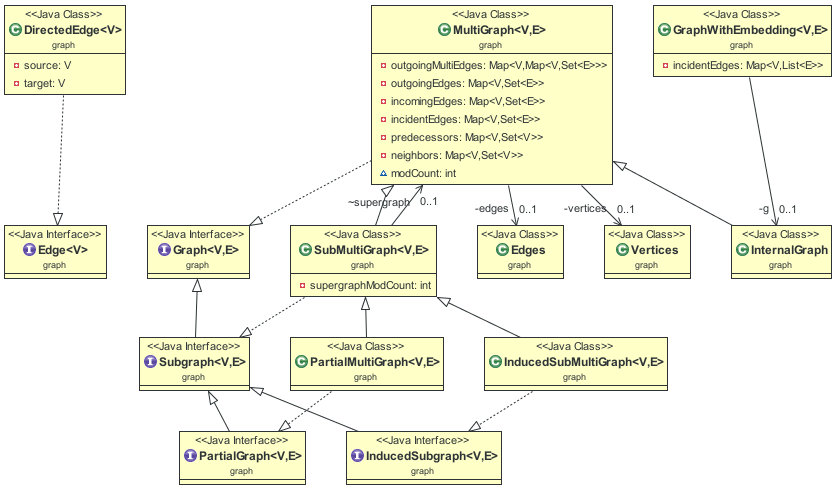
\includegraphics[width=1.05\textwidth]{DiagUML.png}
\caption{\label{fig:DiagUMLPartie1}}
\newline Figure 1: \textit{Diagrammes UML du paquetage "graphe" }}
\end{center}

\newpage
~\\
\subsection{Classe interne, locale et anonyme}

Une classe interne est déclarée à l'intérieur d'une autre classe, Elle peut donc accéder aux variables et méthodes de la classe englobante. Il y a deux modèles principaux de cette dernière, les classes internes statiques qui ne peuvent accéder qu'aux membres statiques de leur classe englobante respective, les classes internes non statiques qui peuvent accéder aux variables et méthodes statiques de leurs classes englobante ainsi qu'a ceux des objets respectifs qui les ont créées.\newline

Une classe interne définie dans un bloc est une classe interne dont la portée est limitée au bloc : c’est une classe interne locale. Une classe locale ne peut pas être statique. Une classe locale peut accéder aux attributs de la classe englobante ainsi qu'aux paramètres et variable locales de la méthode où elle est définie.\newline 

Il est possible de définir une classe interne, sans lui donner de nom par dérivation d'une super classe, ou par implémentation d’une interface, c'est ce qu'on appelle une classe anonyme. Elles sont utiles lorsqu'on a besoin de définir une classe pour ne l'utiliser qu'une seule fois.\newline


\subsection{Correction des warnings}

Au début du stage la bibliothèque contenait de multiples warnings, pour toutes sortes de dysfonctionnement ou de problèmes éventuels. Il fallait retirer ces warnings. Pour cela chaque warning a été traité individuellement selon le problème qui le génère. Pour procéder à cette opération j'ai eu recours à deux solutions : les solutions proposées sur internet et l'utilitaire de réparation des warnings intégré a l'IDE Ecplise.
~\\

\section{Quatrième semaine}

\subsection{Optimisation du code}

Une des éthiques de la programmation est la lisibilité du code, donc j'ai essayé de donner à la bibliothèque un code un peu plus lisible et facile à faire. \newline

Par exemple dans le code j'ai ajouté \texttt{import static graphe.Graph.Edge;} pour avoir \texttt{Edge} au lieu de \texttt{Graph.Edge}.\newline

Pour améliorer la taille du code et sa visibilité, j'ai eu recours à une nouveauté de Java 8 \textbf{les lambda expressions}.

\newpage
~\\
\subsection{Lambda expressions}

Les lambda expressions sont parmi les nouveaux concepts introduits dans Java 8. Leur intérêt est la redéfinition d'une méthode d'une interface fonctionnelle sans avoir à faire une classe anonyme, donc gain de lignes de code et de visibilité.\newline

La sytaxe des lambdas expressions est la suivante :\newline
\textit{(param1, param2, ...) -> \{traitements ; retourne une valeur;\} ;} \newline

Je les ai utilisées dans plusieurs classes de paquetage différents, surtout dans la classe \textit{Iterables} du paquetage \textit{collections} et la classe \textit{RootedSpanningTreelmpl} du paquetage \textit{util}.\newline

\subsection{Entête et licence}

Pour publier un programme (bibliothèque, application, logiciel, ....) développé par soi-même ou en collaboration avec une équipe, il est très important de lui attribuer les copyrights désirés et la licence adéquate, cela permet de protéger le programme et définit avec son cocontractant (exploitant ou utilisateur) les conditions dans lesquelles ce programme peut être utilisé, diffusé ou modifié.\newline

J'ai utilisé l'outil d'Eclipse \textbf{Eclipse copyright Generator}, pour appliquer un commentaire d'en-tête de copyright à tous les fichiers sources dans les projets, ainsi pour ajouter une licence GNU \textbf{Lesser Général Public Licence v3.0} souhaiter par le tuteur de stage.\newline 

Voici une copie de l'en-tête de copyright utilisé dans le projet:\newline

\begin{center}
\textit{Copyright (C) 2018 Olivier Baudon}

\textit{This program is free software: you can redistribute it and/or modify}
\textit{it under the terms of the GNU Lesser General Public License as published by}
\textit{the Free Software Foundation, either version 3 of the License, or}
\textit{(at your option) any later version.}

\textit{This program is distributed in the hope that it will be useful,}
\textit{but WITHOUT ANY WARRANTY; without even the implied warranty of}
\textit{MERCHANTABILITY or FITNESS FOR A PARTICULAR PURPOSE.  See the}
\textit{GNU Lesser General Public License for more details.}

\textit{You should have received a copy of the GNU Lesser General Public License}
\textit{along with this program.  If not, see <http://www.gnu.org/licenses/>.}
\end{center}

\chapter{Bilan du stage} 

\section{Bilan}

Le stage était réparti en deux parties, une première partie théorique et la deuxième pratique.\newline

La partie théorique été très importante pour moi, elle permet de construire une base solide en Java et d'enrichir mes connaissances en théorie des graphes. Dans un premier temps, j'ai consacré mon temps à comprendre en détail les piliers de ce langage, que je connaissais avant, mais je ne le maîtrisais pas bien. Comprendre et maîtriser les exceptions et la généricité est un grand plus à mes connaissances d'informaticien, je les ai trouvés très utiles, cela rendais le code plus souple et robuste.\newline

La partie pratique m'a permis de mettre en oeuvre ce que j'ai apris précédemment. J'ai rencontré quelques difficultés à trouver la bonne syntaxe pour quelques cas, mais ça n'a pas duré avec l'aide du tuteur et de l'internet. Une fois que j'ai appris les lambdas expressions, je les ai trouvées très utiles et facile à mettre en oeuvre. \newline

Ce stage est un grand plus moi, en premier lieu j'ai apris à comprendre un code déjà écrit et savoir le modifier/améliorer sans affecter les autres parties du programme, ainsi que maitriser beaucoup mieux la programmation orientée objet, en utilisant le langage Java. J'ai apris aussi à utiliser les plugins pour accélérer le rythme du travail, tel que les outils pour tracer des diagrammes UML ou pour générer les copyright/licences.\newline

J'ai écrit ce rapport en utilisant \LaTaX. Je connaissais déjà cet outile mais je ne le maitrisais pas bien. Ecrire mon premier rapport de stage en utilisant ce système de composition de documents, m'a permit d'avoir une meilleure connaissance sur \LaTeX, et de réaliser son importance à automatiser le travaille et d'améliorer l'écriture des formules scientifique, ansi que réduire le temps de rédaction des documents.


\begin{comment}
1) ajout des commentaires 
2) java doc 
3) ilustrer avec des exemples
\end{comment}


\newpage
\section{Référence}
\begin{verbatim}
https://openclassrooms.com/courses/apprenez-a-programmer-en-java/
les-classes-abstraites-et-les-interfaces

https://openclassrooms.com/courses/apprenez-a-programmer-en-java/
les-exceptions

http://thecodersbreakfast.net/index.php?post/2008/07/23/77-java-les-var-args

https://openclassrooms.com/courses/apprenez-a-programmer-en-java/
les-collections-d-objets

http://objectaid.com/

http://imss-www.upmf-grenoble.fr/prevert/Prog/Java/CoursJava/classes3.html

https://openclassrooms.com/courses/apprenez-a-programmer-en-java/classes-anonymes-interfaces-fonctionnelles-lambdas-et-references-de-methode

https://jmini.github.io/Eclipse-Copyright-Generator/

https://fr.wikipedia.org/wiki/Licence_de_logiciel
\end{verbatim}

\end{document}
